\documentclass[12pt,a4]{article}

\usepackage{polski}
\usepackage[utf8]{inputenc}
\usepackage{graphicx}

\title{Konspekt realizacji zadania}
\author{Łukasz Ślusarczyk}

\begin{document}

\maketitle
\tableofcontents
\clearpage

\section{Wstęp}
Niniejszy konspekt opisuje przedmiot i sposób badania, a także
proponowane rozwiązanie. Dokument zawiera opis programu od strony
użytkownika, jednak bez szczegółowego opisu interfejsu.

\section{Badany problem - przewidywanie parametrów ruchu obrotowego
Ziemi}

\indent Tematem pracy będzie przewidywanie parametrów ruchu obrotowego
ziemi (w skrócie \emph{EOP}, czyli \emph{Earth Orientation Parameters})
zbieranych przez Międzynarodową Unię Astronomiczną, a dokładniej przez
organizację IERS\footnote{International Earth Rotation Service - http://www.iers.org}.
Udostępnia ona między innymi historyczne dane dziennych pomiarów EOP.
Dzienne dane były rejestrowane rejestrowanie od 1962 roku, z tym że wcześniejsze dane mają
mniejszą dokładność. Dane które chciałbym przetwarzać sieciami neuronowymi
są dostepne na stronie:
\begin{verbatim}
http://www.iers.org/nn_11252/SharedDocs/MetaDaten
/11221__EOP__C04__05__62__NOW__IAU2000A.html
\end{verbatim}
\indent Znaczenie tych danych jest następujące. Na ruch ziemi, czy ona
kręci się szybciej czy wolniej, i gdzie aktualnie przebiega oś obrotu ziemi,
na to wszystko wpływa wiele czynników. Te najważniejsze są znane -
ruch księżyca, innych planet, odległość od słońca, rozkład gęstości masy we
wnętrzu ziemi, nasza wiedza o tym gdzie jest płynne jądro, a gdzie
stałe itd. Te wszystkie rzeczy są zebrane w tak zwanych \emph{modelach
referencyjnych}. Jednym z takich modeli, uwzględniających
najnowszą wiedzę o czynnikach wpływających na ruch naszej planety jest
model \emph{IAU2000 C04 05}. Ten model opisuje jak powinna się obracać ziemia. 
W rzeczywistości gdy mierzymy parametry ruchu obrotowego, ziemia obraca się nieco inaczej i
odstępstwa od modelu, zwane \emph{residuami}, są właśnie zebrane w
pliku z linku powyżej.\\
\indent Przewidywanie jak te odstępstwa będą wyglądały w najbliższych kilku
dniach będzie właśnie zadaniem projektowanej sieci neuronowej.

\section{Istniejące podejścia do rozwiązania problemu}

\indent Przewidywanie EOP jest badane na wiele różnych sposobów i
wykorzystuje się głównie techniki znane z przetważania sygnałów,
modele autoregresji, korelację, koherencję, transformaty falkowe. Są
też próby prognozowania EOP za pomocą sieci neuronowych.\\
\indent Jedną z publikacji na ten temat jest praca \emph{Prediction of Earth
orientation parameters by artificial neural networks - H. Schuh, M.
Ulrich, D. Egger, J. Muller, W. Schwegmann}\footnote{Journal of Geodesy
(2002) 76: 247-258,\\http://www.springerlink.com/content/vu1fk2krt918u32g/}
Wykorzytywane sieci neuronowe nie są tam jednak wyrafinowane. Jest to
jedynie MLP i nie specjalnie formalnie optymalizowane w poszukiwaniu
najlepszej struktury sieci.\\
\indent Inną pracą jest plakat o zastosowaniu sieci neuronowych do
badania EOP w zestwieniu ze stosowaniem modeli autoregresji oraz
metody najmniejszych kwadratów: \emph{NN in EOP prediction - M. Kalarus}
\footnote{http://www.cbk.waw.pl/~kalma/presentations/Application\_of\_NN\_EGU2005.pdf}.
Mam wrażenie, że autor plakatu z pierwszego linku zrobił wszystko dokładnie tak jak to jest
opisane we wcześniej wspomnianej publikacji, a dodał tylko porównanie
z innymi metodami przewidywania EOP.

\section{Proponowane rozwiązanie}

\subsection{Rodzaj sieci}
Do rozwiązania problemu zostanie użyta sieć RMLP - Recurrent Multi
Layer Percepton. Planuję porównać otrzymane za jej pomocą wyniki z
wynikami publikacji H. Schuh'a.

\subsection{Optymalizacja struktury}
W rozdziale 4.3 książki S. Osowskiego, są opisane soposoby optymalnego
doboru architektury sieci pod względem generalizacji poprzez bądź to
usuwanie najmniej aktywnych neuronów, bądź
budowanie kilku sieci i braniu średniej ważonej wyników każdej z nich.
Chciałbym również zastosować jeden z tych algorytmów w poszukiwaniu
optymalnej struktury sieci.

\subsection{Badany parametr - długość dnia}
Z parametrów ruchu obrotowego ziemi, tj współrzędnych bieguna,
różnicy czasu UTC i UT1, długości dnia, wybrałbym jednowymiarową
długość dnia\footnote{LOD - length of day}. 
Wyniki dla niej są podane w ww publikacji tak, że
można mieć porównanie jak dobrze przewiduje się tę wielkość.

\subsection{Metoda uczenia i opis wejścia/wyjścia sieci}
Sieć będzie uczona w trybie online z nadzorem. Dane zostaną podzielone w stosunku
1:1:4 na dane weryfikujące, testujące i uczące. Na danych testujących
będzie poszukiwane minimum odchylenia średniokwadratowego.\\
\indent Wejściem będzie parametr LOD dla danego dnia, wyjściem będzie
czwórka liczb prezentująca przewidywane długości dni o 1,2,3,5 w
przód. Preprocessing wejściowych danych nie będzie potrzebny, one są
już preprocesowane przed umieszczeniem ich na stronie w celu
wyeliminowania wysokoczęstotliwościowego szumu. Podstawowe statystyki
liczbowe danych wejściowych są przedstawione w publikacji H. Schuha.
Nie ma obserwacji niepełnych. Liczba obserwacji pełnych jest równa
około 18 tysięcy, co odpowiada dziennym pomiarom od 1962 roku.
Dane wejściowe są przedstawione na rysunku \ref{fig:lod}.

\begin{figure}[htbp]
  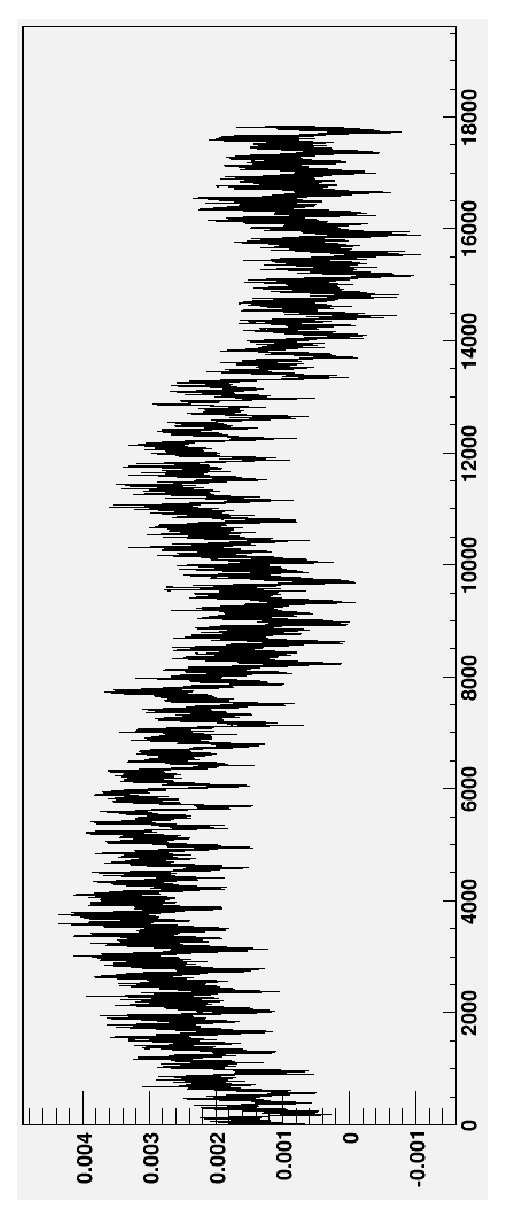
\includegraphics[]{doc/img/lod.eps}
  \caption{Dane wejściowe, mierzone odstępstwa od długości dnia w sekundach}
  \label{fig:lod}
\end{figure}

\end{document}

%    * z jakiej sieci korzystamy
%        * jaką metodę/metody uczenia wykorzystujemy
%	    * jak uczymy na danych - co jest na wejściu sieci, a co na
%	    wyjściu
%	        * z jakich danych korzystamy (krótki opis: dziedzina,
%		liczba atrybutów, rodzaj atrybutów, czy potrzebny jest
%		preprocessing itp.) i skąd bierzemy te dane (np. nazwa
%		i adres repozytorium internetowego)
%		    * dla badanych danych (chodzi tu o dane wejściowe,
%		    na których działa badany algorytm) przedstawienie
%		    podstawowych statystyk liczbowych (liczba
%		    atrybutów; mediana, średnia, odchylenie
%		    standardowe, max, min dla każdego atrybutu) i
%		    graficznych (histogramy, wykresy zależności par
%		    zmiennych, wykresy warunkowe). Podać liczbę
%		    obserwacji niepełnych (nie posiadających wartości
%		    dla jednego z atrybutów) i liczbę obserwacji
%		    niepełnych dla danego atrybutu. Można również
%		    poddać liczbę obserwacji niepełnych dla każdej z
%		    klas występujących w danych. Celem jest tutaj
%		    bliższe zapoznanie się z danymi, z których będziemy korzystać.
		    
		    
